\documentclass[lettersize,journal]{IEEEtran}

% *** CITATION PACKAGES ***
\usepackage{cite}
\usepackage{graphicx}
\usepackage{enumitem}
\usepackage{listings}
\usepackage{amsmath,amssymb} 
\usepackage{subcaption}
% \renewcommand*{\figureautorefname}{Fig.} 
\graphicspath{{figures/}}
\DeclareGraphicsExtensions{.jpg}

 
 
% \usepackage[caption=false,font=footnotesize]{subfig} 


% *** PDF, URL AND HYPERLINK PACKAGES ***
\usepackage{hyperref}  
\hypersetup{
    colorlinks=true,
    linkcolor=blue,    
    urlcolor=cyan, 
}


\begin{document}

\title{Lab 2 - Noise Removal \\ \vspace{0.1em} \LARGE Computational Vision \& Imaging}

\author{\textbf{Student ID}: XXXXXXX \\
~\IEEEmembership{Random Student,~School of Computer Science,\\University of Birmingham, UK, B15 2TT}
% <-this % stops a space
\thanks{This is a solution for the Formative Assignment by Hamid Dehghani}
% <-this % stops a space
\thanks{The report was submitted to Canvas on Feb 23 and reviewed by a TA}}

% The paper headers
\markboth{Collection of Lab Reports, Computer Vision, No.~2, February~2022}%
{Shell \MakeLowercase{\textit{et al.}}: A collection of Report submissions documenting assignment solutions}

\maketitle

\begin{abstract}
This document is a formal solution for the Lab 2 Formative Assignment based on Noise Removal. It shows how Gaussian filters can be applied to remove noise form the image and how different parameters (e.g., standard deviation, kernel size) impact the output. It also performs tests on time and checks how Laplacian filter works.
\end{abstract}

\begin{IEEEkeywords}
Lab 2, formative assignment, computer vision, imaging, noise removal, filters, kernels, Sobel, Laplacian, Gaussian, MATLAB.
\end{IEEEkeywords}

\section{Introduction}
\IEEEPARstart{C}{ontinuing} the previous topic of \emph{Edge Detection}, we were shown that it can be enhanced by removing the noise from the image. In other words, a filter can be applied to average out abrupt gradient changes which will smoothen the noise. After that, an edge filter can be applied and we can hope to see better results. Often, they depend on the parameters of the noise reduction filter, which most commonly is chosen as Gaussian filter.

\section{Setup}
We continue the setup of the 1st lab with our working image "shakey.150.gif". In MATLAB, we are additionally provided with Gaussian 3x3 and 5x5 filter. Specific values are not necessary important, what should be noted is that such filters have largest weight on the middle value and smaller weights on the surrounding values. It can be generated using formula \ref{eq:1} (note that $1 \leq i, j \leq (2k + 1)$).

\begin{equation}\label{eq:1}
    H_{ij}= \frac{1}{2\pi\sigma^2}\exp \left(-\frac{(i-(k+1))^2+(j-(k+1))^2}{2\sigma^2} \right)
\end{equation}

We are provided with "N.m" function which calculates a \emph{Gaussian} vector given a mean, a sigma value and a range. The \emph{Gaussian} kernel then can be produced as an outer product of the 2 vectors. We are also given a \emph{Laplacian} filter which is shown by equation \ref{eq:2}.

\begin{equation}\label{eq:2}
    \text{Laplacian}=\begin{bmatrix}0 & 1 & 0 \\ 1 & -4 & 1 \\ 0 & 1 & 0\end{bmatrix}
\end{equation}

\emph{Laplacian} is essentially the sum of second order derivatives. For change in $x$, we take the difference between the differences involving the center and adjacent pixels for that row, for change in $y$ - involving centre and adjacent pixels in that column. I. e., in our 3-by-3 case, the second order derivative with respect to $x$ and $y$ can be shown by \autoref{eq:3} and \autoref{eq:4}.

\begin{equation}\label{eq:3}
    \begin{array}{l@{{}={}}l}
        (\nabla_{x^2}^2I)_{h,w} & (I_{h,w+1}-I_{h,w}) - (I_{h,w} - I_{h,w-1}) \cr & I_{h,w-1}-2I_{h,w}+I_{h,w+1}
    \end{array}
\end{equation}

\begin{equation}\label{eq:4}
    (\nabla_{y^2}^2I)_{h,w}=I_{h-1,w}-2I_{h,w}+I_{h+1,w}
\end{equation}

We are also required to use \emph{zerocrossing} method at some point which is provided by MATLAB via built-in "edge" function. \emph{Zerocrossing} essentially means detecting those points where a sign of a value changes. Regarding our functions in assignment 1, we will reuse  magnitude and error calculations.

\section{Analysis Part 1}
\subsection{Step 1}\label{subsection:1:1}
\noindent Step 1 asks to experiment with the provided 3x3 and 5x5 \emph{Gaussian} filters.

\hbox{}

\noindent\textbf{Question}: can you see any difference between them?

\hbox{}

\noindent\textbf{Answer}:  the convolved image with the 5x5 filter is more blurry, thus smoother, than with the 3x3 filter. This is because a larger filter is applied to a larger local area and it makes it more similar to the surrounding pixels because more pixels influence the convolved value than a few specific ones.

\begin{figure}[h]
    \centering 
     
    \begin{subfigure}[h]{0.23\textwidth}
        \centering 
        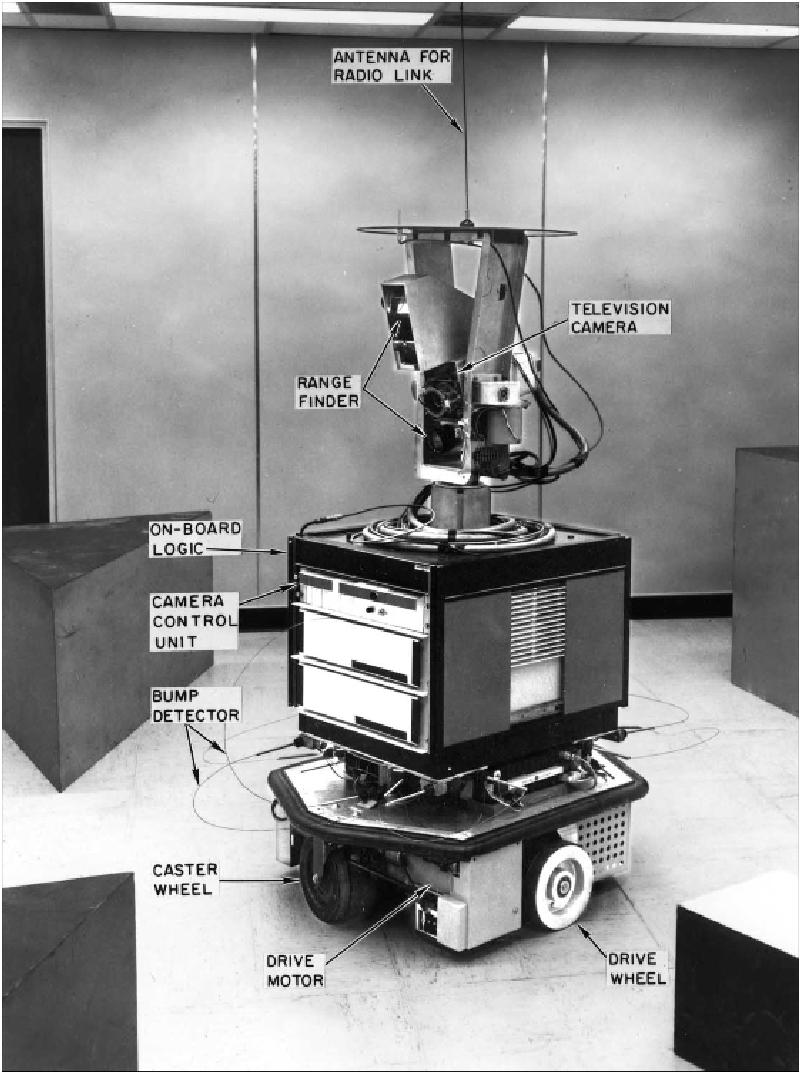
\includegraphics[width=\linewidth]{gaussian_3x3_map}
        \caption{3x3 Gaussian filter}  
    \end{subfigure}
    % \hfill
    \begin{subfigure}[h]{0.23\textwidth}
        \centering
        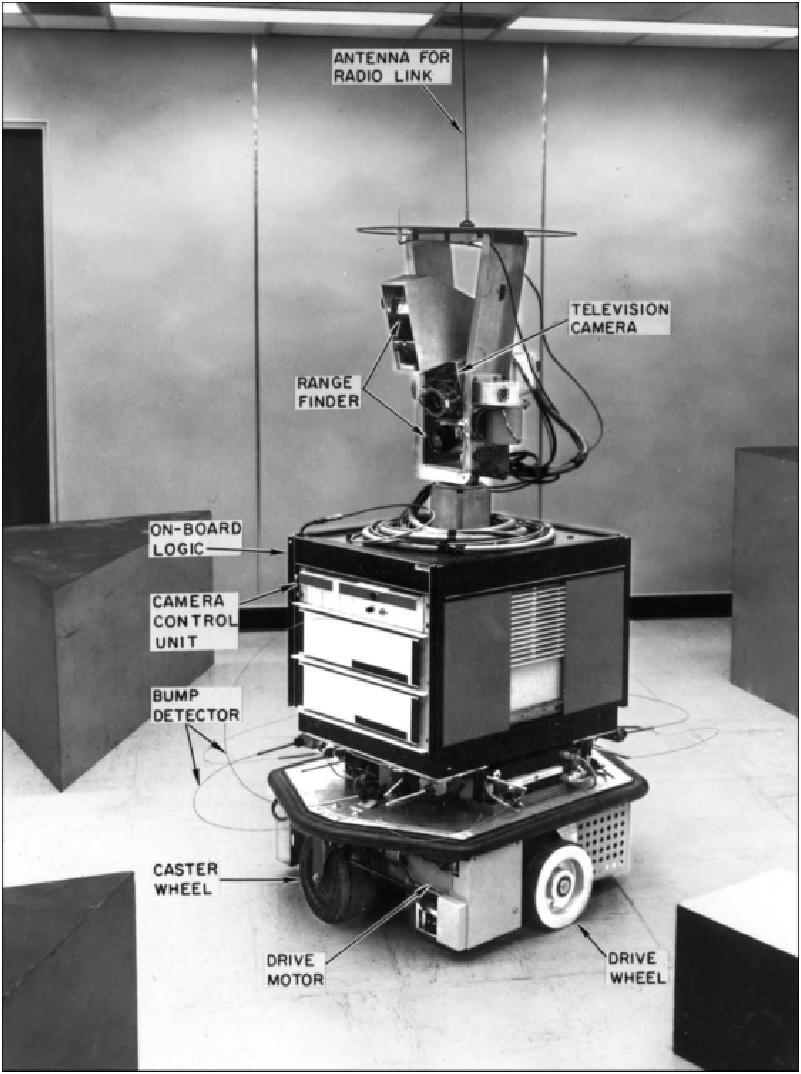
\includegraphics[width=\linewidth]{gaussian_5x5_map}
        \caption{5x5 Gaussian filter}  
    \end{subfigure}
    % \hfill 
    \caption{Image convolved with different Gaussian filters}
    \label{fig:1}
\end{figure}

\newpage

\noindent\textbf{Task}: try applying an edge filter to each and thresholding.

\hbox{}

\noindent\textbf{Results}: the edge map acquired by applying an edge filter on a 5x5 Gaussian map has less noise. This is due to the fact that the larger filter smoothens the image better than the small filter (i.e., the same reason as above).

\begin{figure}[h]
    \centering 
    \begin{subfigure}[h]{0.155\textwidth}
        \centering 
        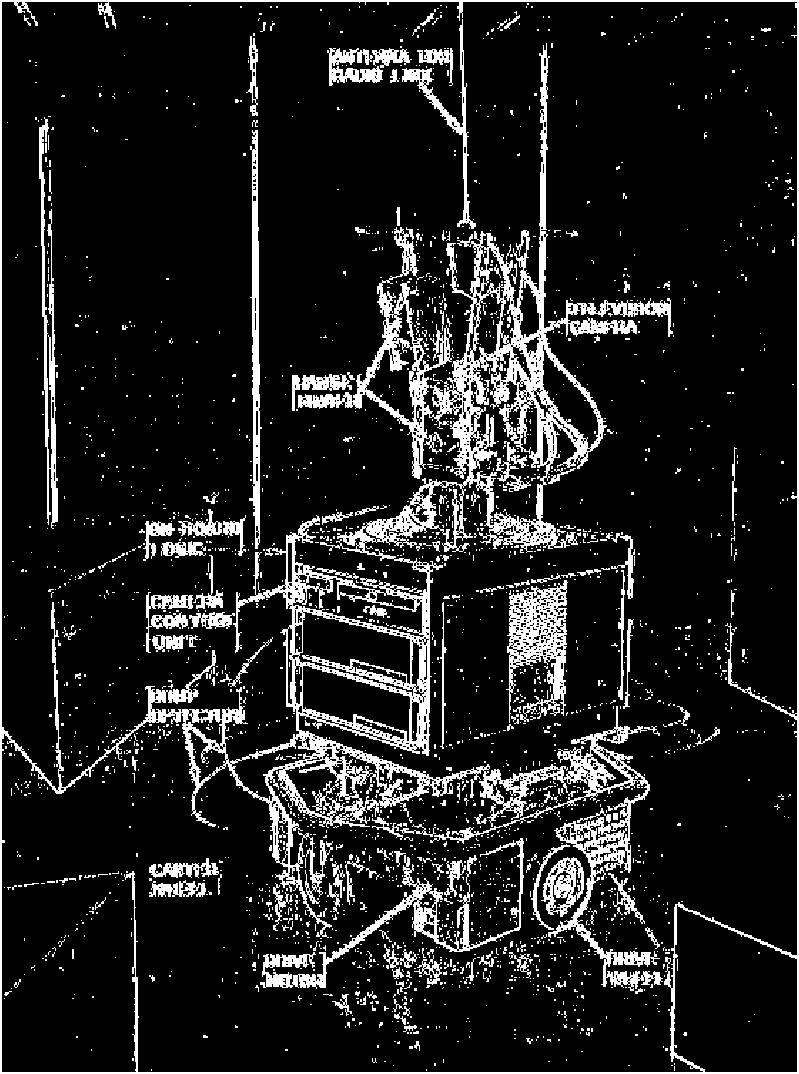
\includegraphics[width=\linewidth]{sobelX_map}
        \caption{SobelX}  
    \end{subfigure}
    % \hfill
    \begin{subfigure}[h]{0.155\textwidth}
        \centering 
        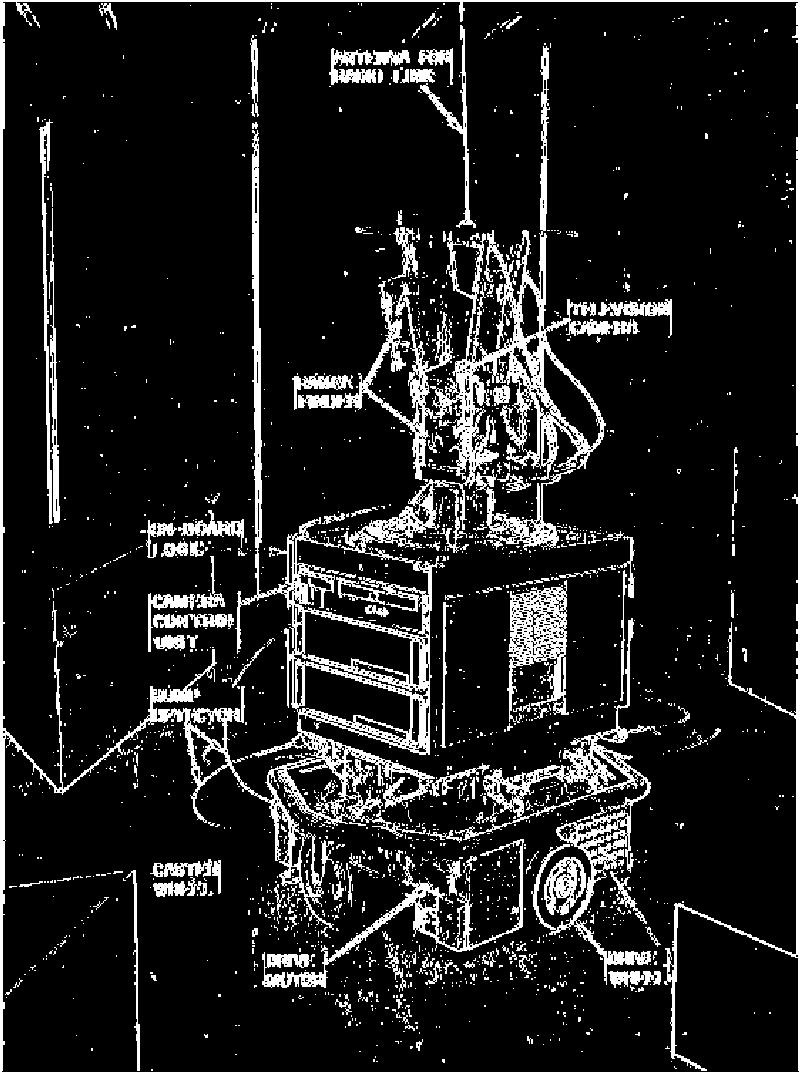
\includegraphics[width=\linewidth]{gaussian_3x3_sobelX_map}
        \caption{3x3 + SobelX}  
    \end{subfigure}
    % \hfill
    \begin{subfigure}[h]{0.155\textwidth}
        \centering
        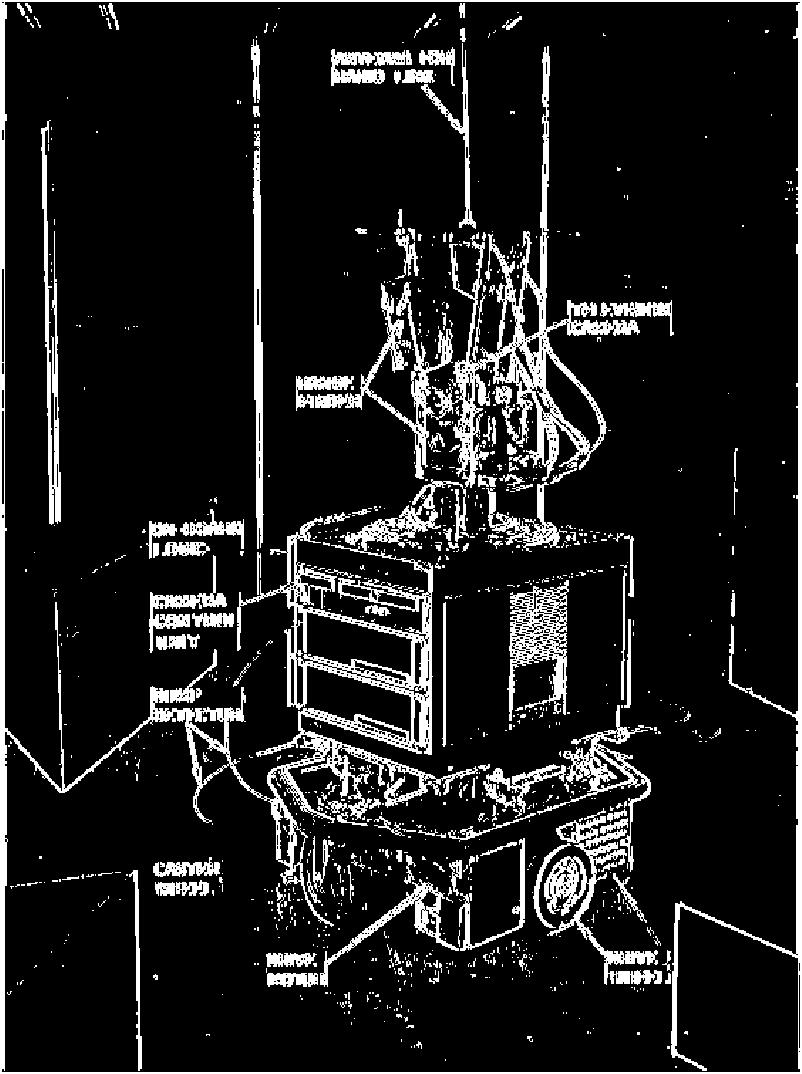
\includegraphics[width=\linewidth]{gaussian_5x5_sobelX_map}
        \caption{5x5 + SobelX}  
    \end{subfigure}
    % \hfill 
    \caption{Pure image and 2 blurred maps from figure \autoref{fig:1} convolved with a horizontal Sobel filter and thresholded at 40}
    \label{fig:2}
\end{figure}

\subsection{Task 1}\label{subsection:1:2}

\noindent Task 1 asks to compare the pure image convolved with an edge filter with blurred images convolved with an edge filter.

\hfill

\noindent\textbf{Question}: can you describe the effect in comparison with applying the edge filter to the image directly?

\hfill

\noindent\textbf{Answer}: considering the same threshold, if we we apply the edge filter directly on the image, there will be more noise in the acquired map, i.e., visually more false positives are captured as edges. In contrast, smoothening the image with a \emph{Gaussian} filter prior to applying an edge filter averages the noise out and keeps the edges more standing out. However, a trade-off can be seen as well between edge details and noise. The effects can be seen in \autoref{fig:2}.

\section{Analysis Part 2}

\subsection{Step 2}\label{subsection:2:1}

\noindent Step 2 asks to create different Gaussian masks and see what happens to the output as the parameters of the generating function change. It also asks to apply an edge filter and inspect the results.

\hfill

\noindent\textbf{Question}: what happens to the image as you increase the size of the mask? What happens as you increase the size of \textbf{s} ($\sigma$)?

\hfill

\noindent\textbf{Answer}: as we increase the size of the mask, the image becomes more blurry (similar reason explained in \autoref{subsection:1:1}) This effect can be observed in \autoref{fig:3}. As we increase standard deviation, the image also becomes more blurry because the weight values become more spread around the mean, thus surrounding cells play a bigger role in the local area when it is convolved with the kernel. This effect can be observed in \autoref{fig:4}.

\begin{figure}[h]
    \centering 
    \begin{subfigure}[h]{0.115\textwidth}
        \centering 
        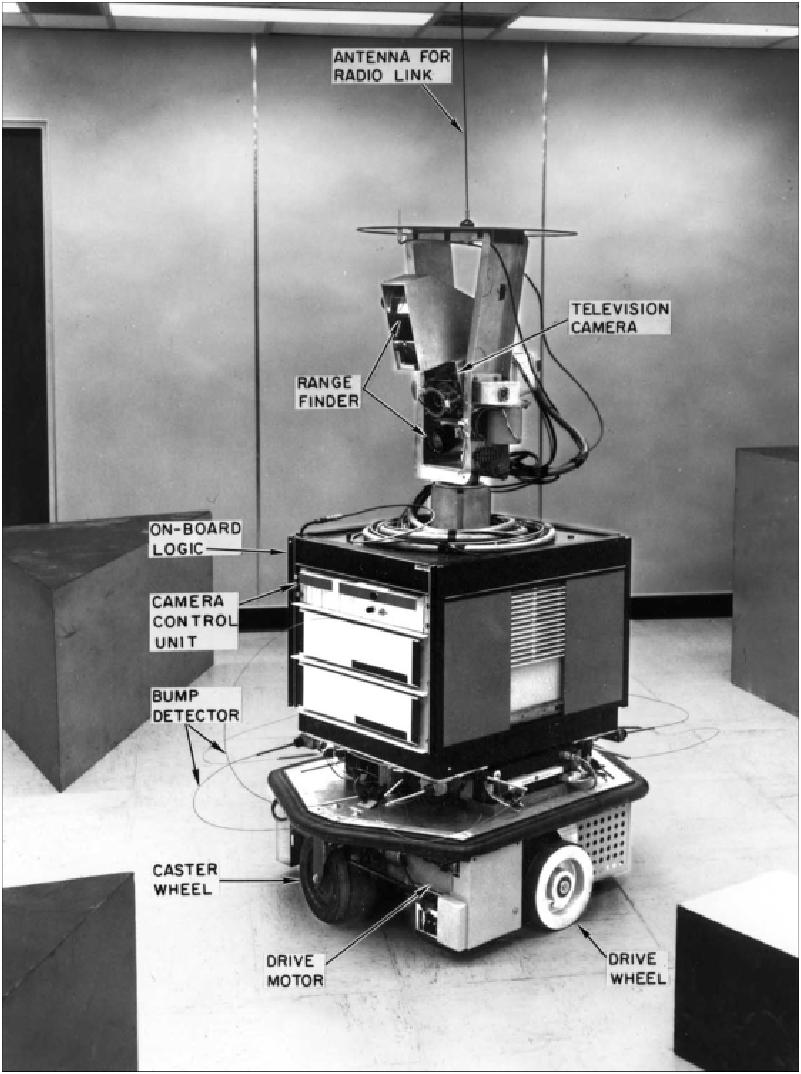
\includegraphics[width=\linewidth]{gaussian_map_3x3_sigma_1}
        \caption{3x3}  
    \end{subfigure}
    % \hfill
    \begin{subfigure}[h]{0.115\textwidth}
        \centering 
        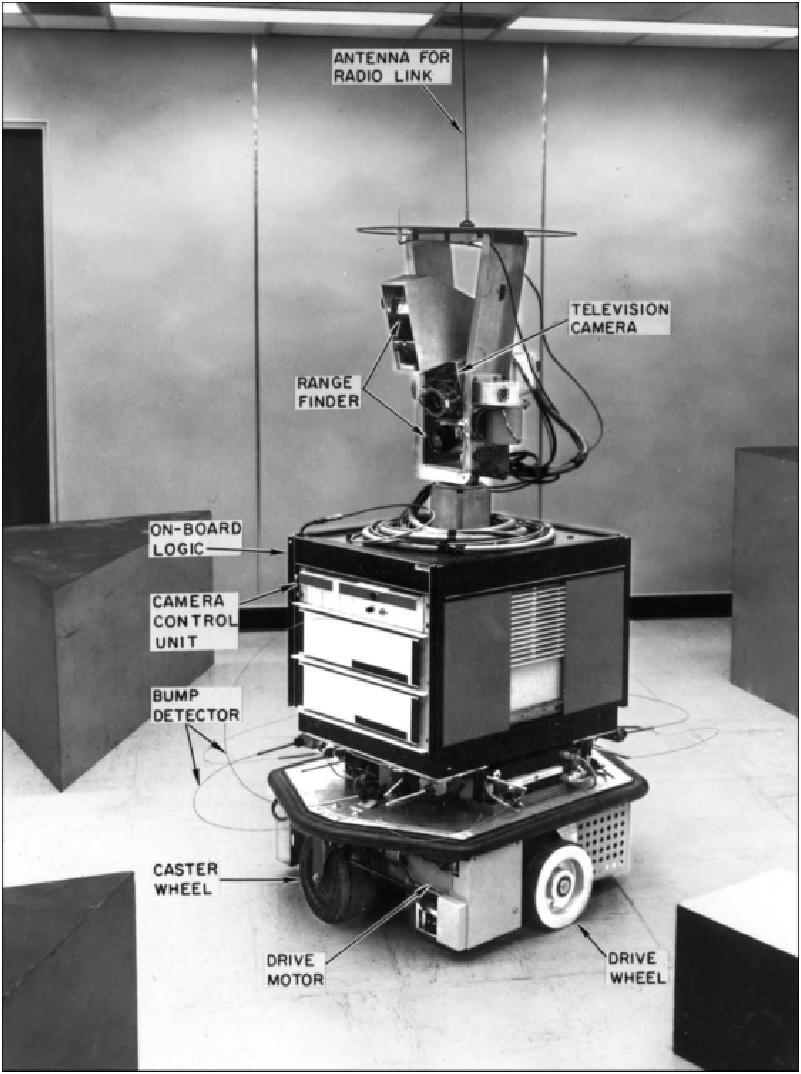
\includegraphics[width=\linewidth]{gaussian_map_5x5_sigma_1}
        \caption{5x5}  
    \end{subfigure}
    % \hfill
    \begin{subfigure}[h]{0.115\textwidth}
        \centering
        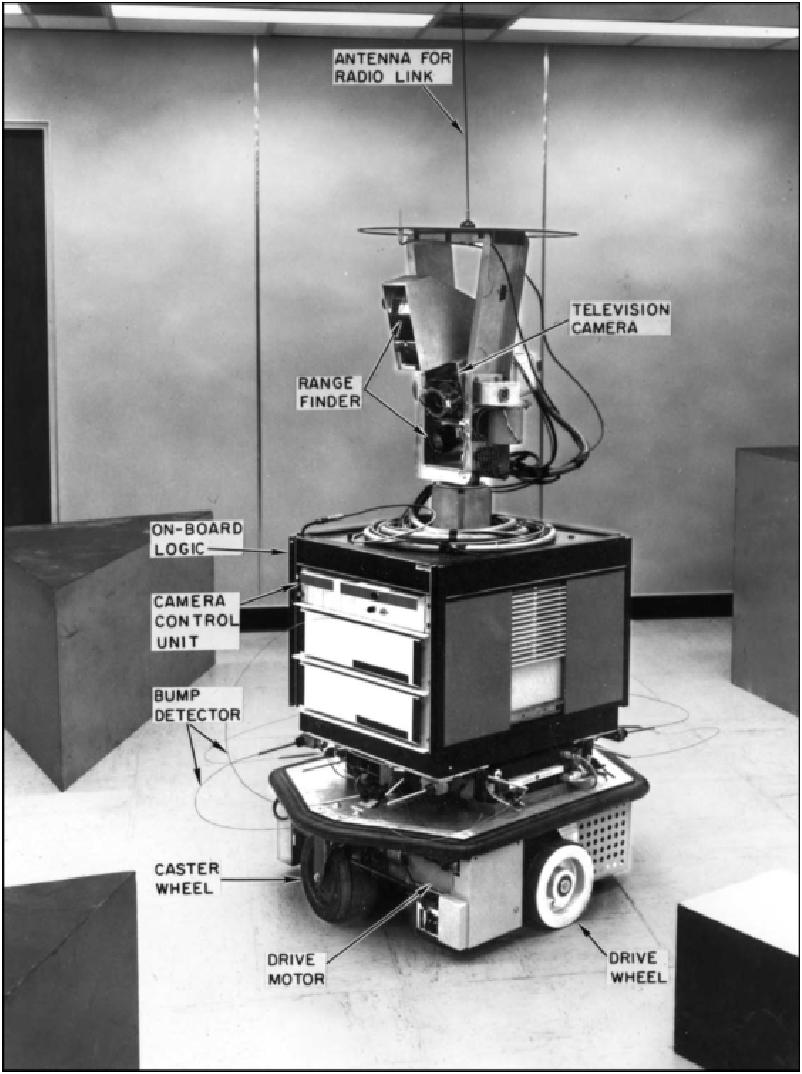
\includegraphics[width=\linewidth]{gaussian_map_7x7_sigma_1}
        \caption{7x7}  
    \end{subfigure}
    % \hfill
    \begin{subfigure}[h]{0.115\textwidth}
        \centering
        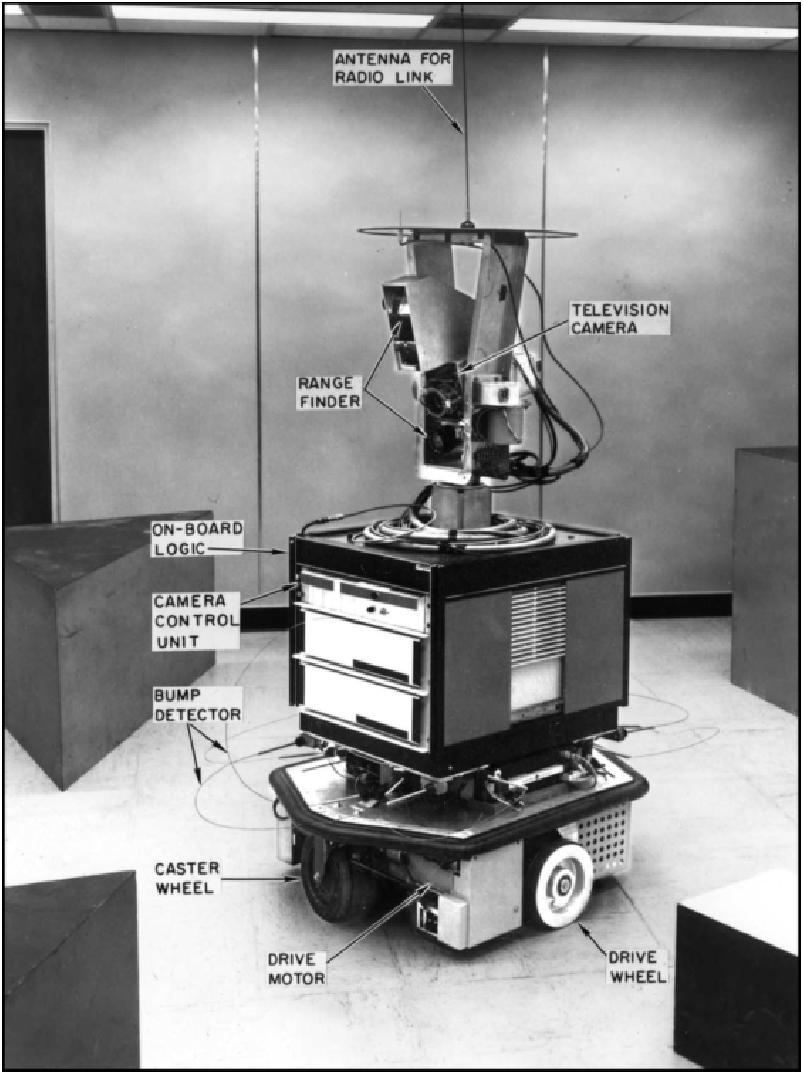
\includegraphics[width=\linewidth]{gaussian_map_9x9_sigma_1}
        \caption{9x9}  
    \end{subfigure}
    \begin{subfigure}[h]{0.115\textwidth}
        \centering 
        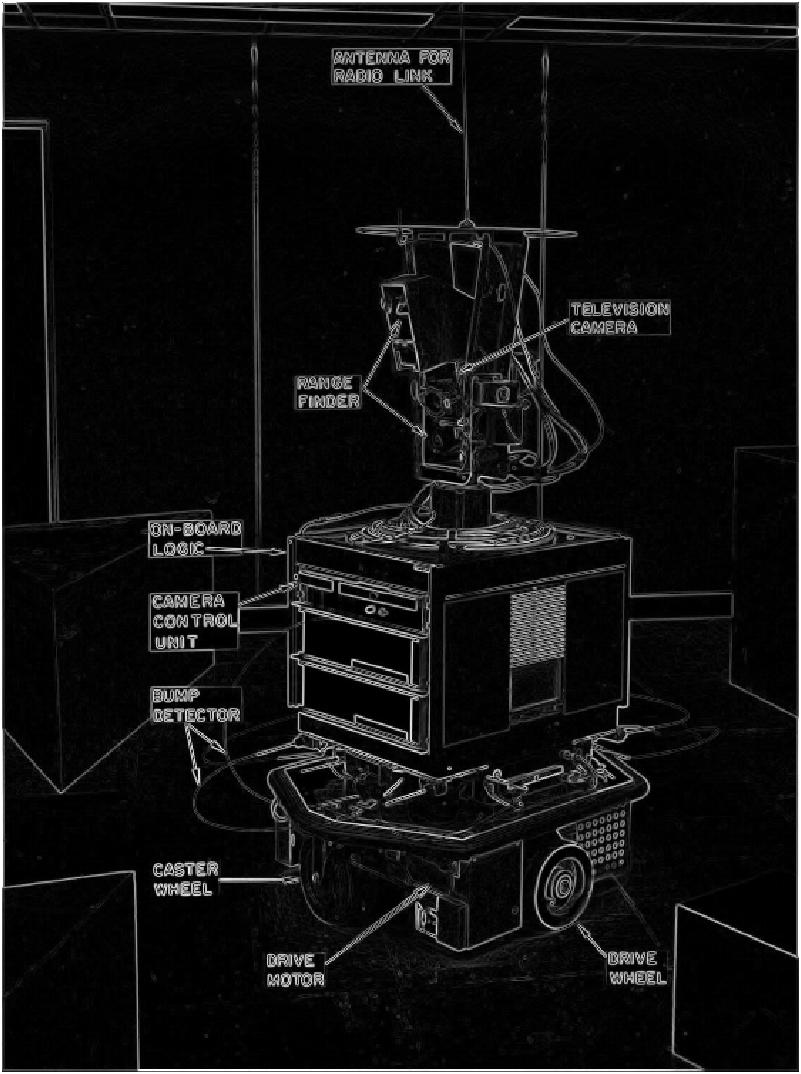
\includegraphics[width=\linewidth]{gaussian_edge_map_3x3_sigma_1}
        \caption{3x3}  
    \end{subfigure}
    % \hfill
    \begin{subfigure}[h]{0.115\textwidth}
        \centering 
        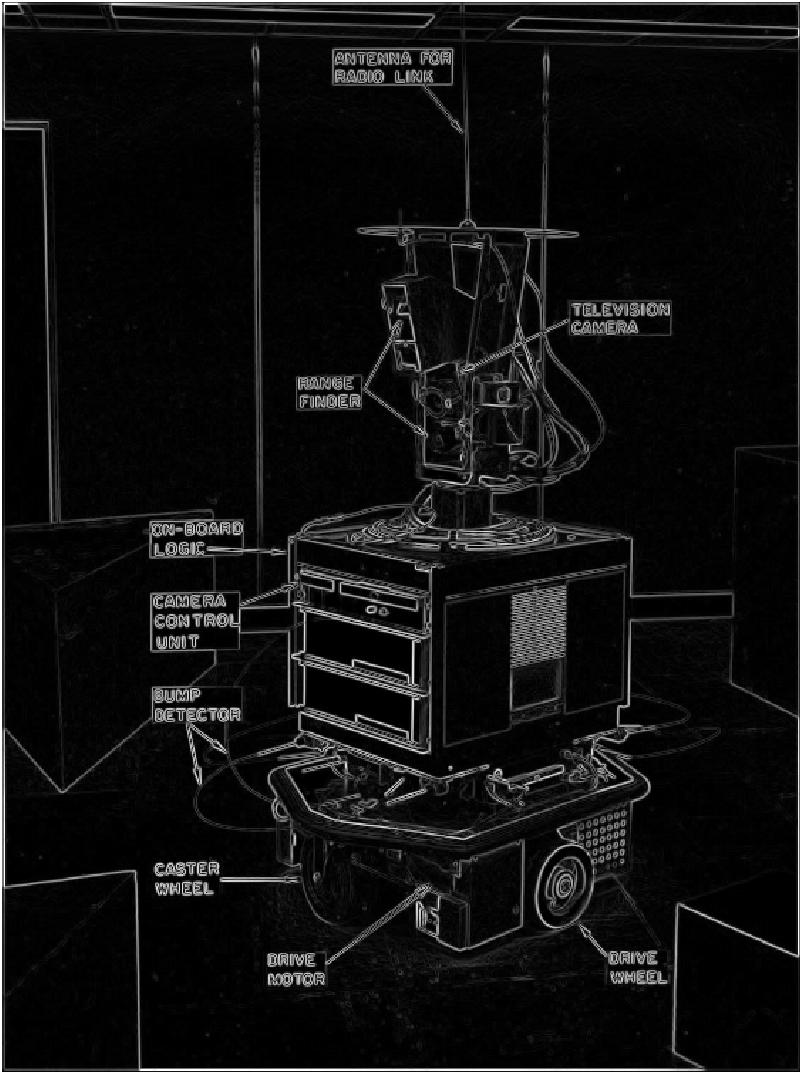
\includegraphics[width=\linewidth]{gaussian_edge_map_5x5_sigma_1}
        \caption{5x5}  
    \end{subfigure}
    % \hfill
    \begin{subfigure}[h]{0.115\textwidth}
        \centering
        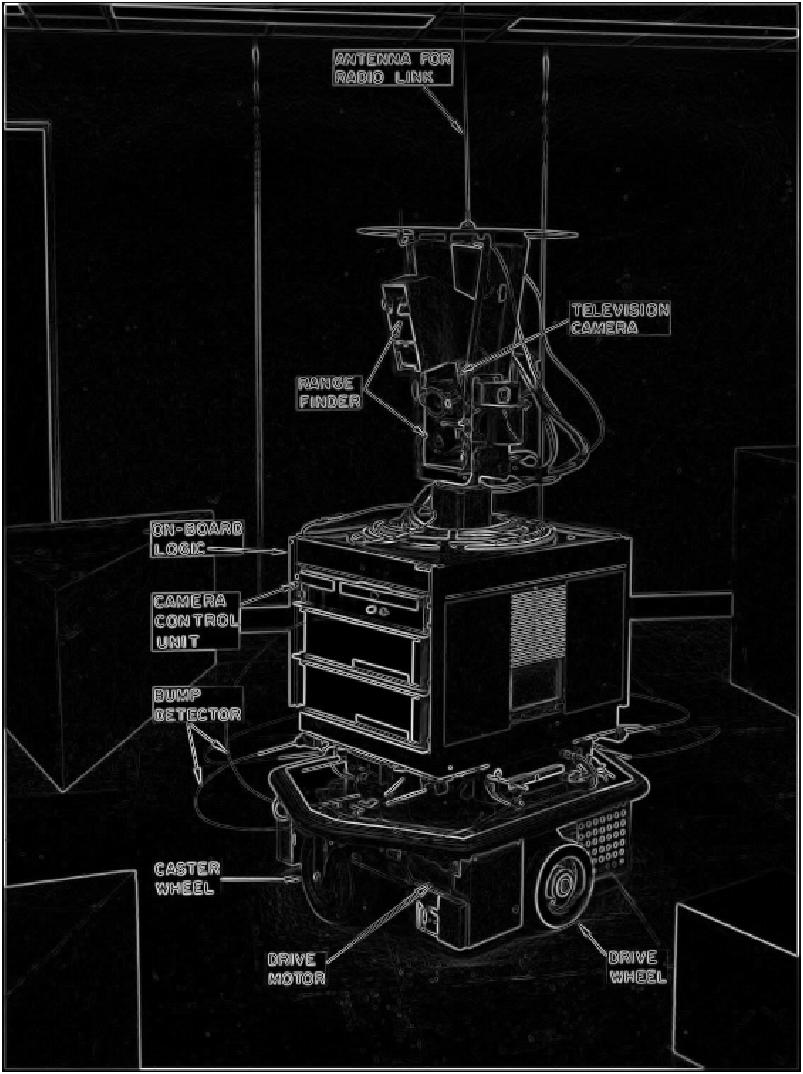
\includegraphics[width=\linewidth]{gaussian_edge_map_7x7_sigma_1}
        \caption{7x7}  
    \end{subfigure}
    % \hfill
    \begin{subfigure}[h]{0.115\textwidth}
        \centering
        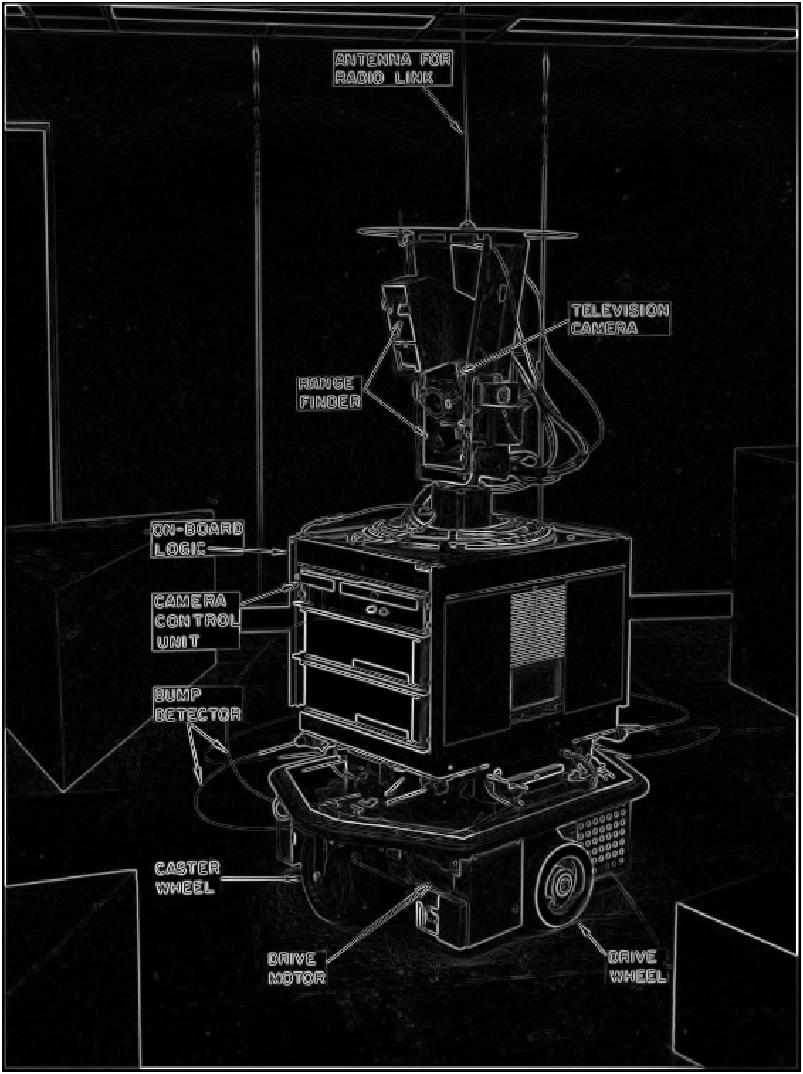
\includegraphics[width=\linewidth]{gaussian_edge_map_9x9_sigma_1}
        \caption{9x9}  
    \end{subfigure}
    \caption{Experiments with different Gaussian filter sizes while keeping $\sigma=1$. The top row contains pure images on which the Gaussian filters were applied. The bottom row contains the top row images but on which the horizontal and vertical Sobel filters were applied and the magnitude was calculated}
    \label{fig:3}
\end{figure}

\begin{figure}[h]
    \centering 
    \begin{subfigure}[h]{0.115\textwidth}
        \centering 
        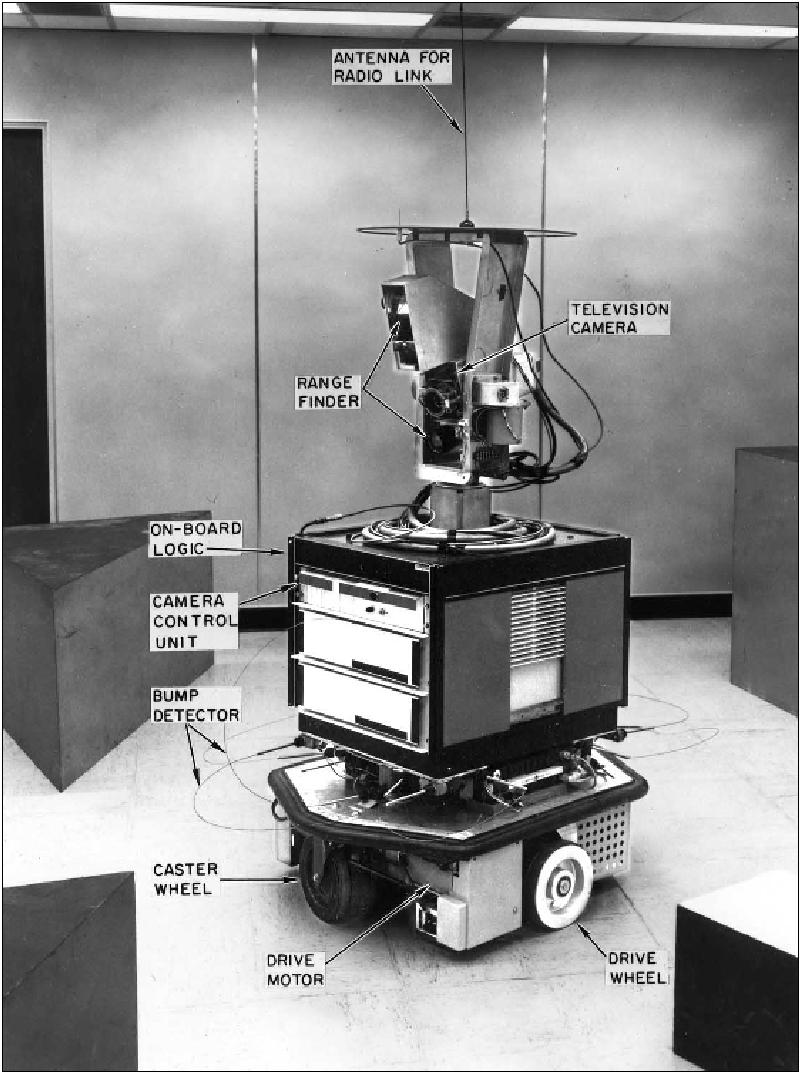
\includegraphics[width=\linewidth]{gaussian_map_5x5_sigma_0.1}
        \caption{$\sigma=0.1$}  
    \end{subfigure}
    % \hfill
    \begin{subfigure}[h]{0.115\textwidth}
        \centering 
        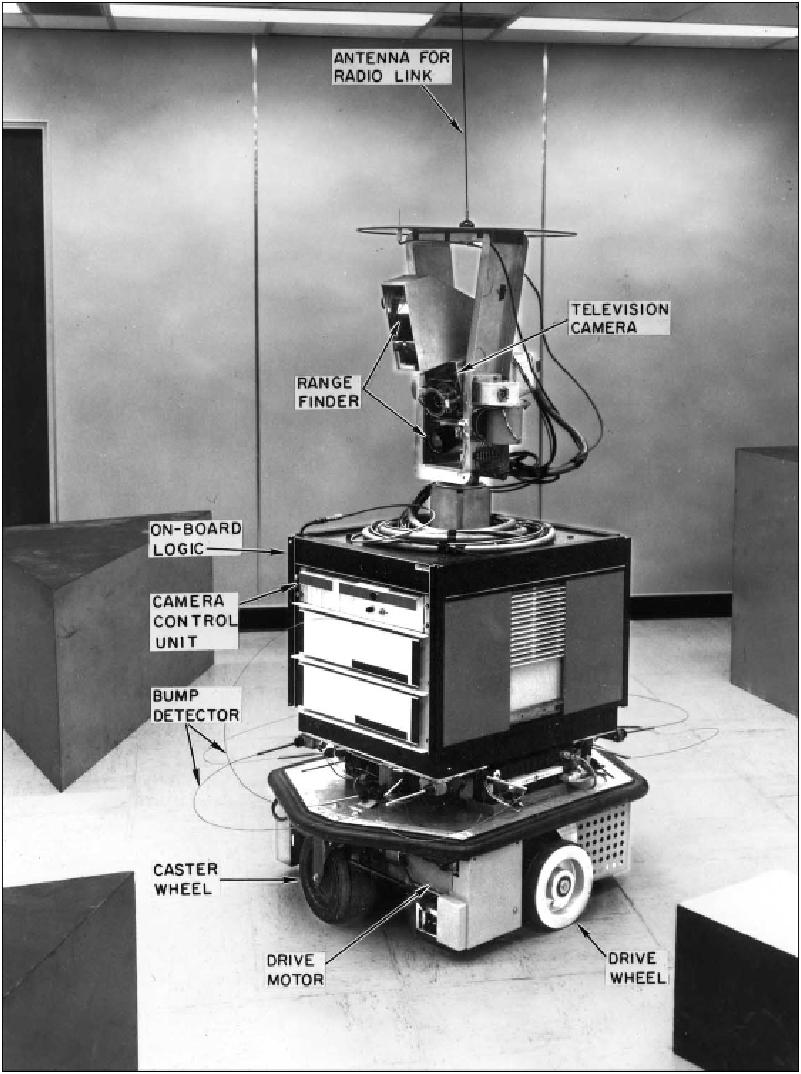
\includegraphics[width=\linewidth]{gaussian_map_5x5_sigma_0.5}
        \caption{$\sigma=0.5$}  
    \end{subfigure}
    % \hfill
    \begin{subfigure}[h]{0.115\textwidth}
        \centering
        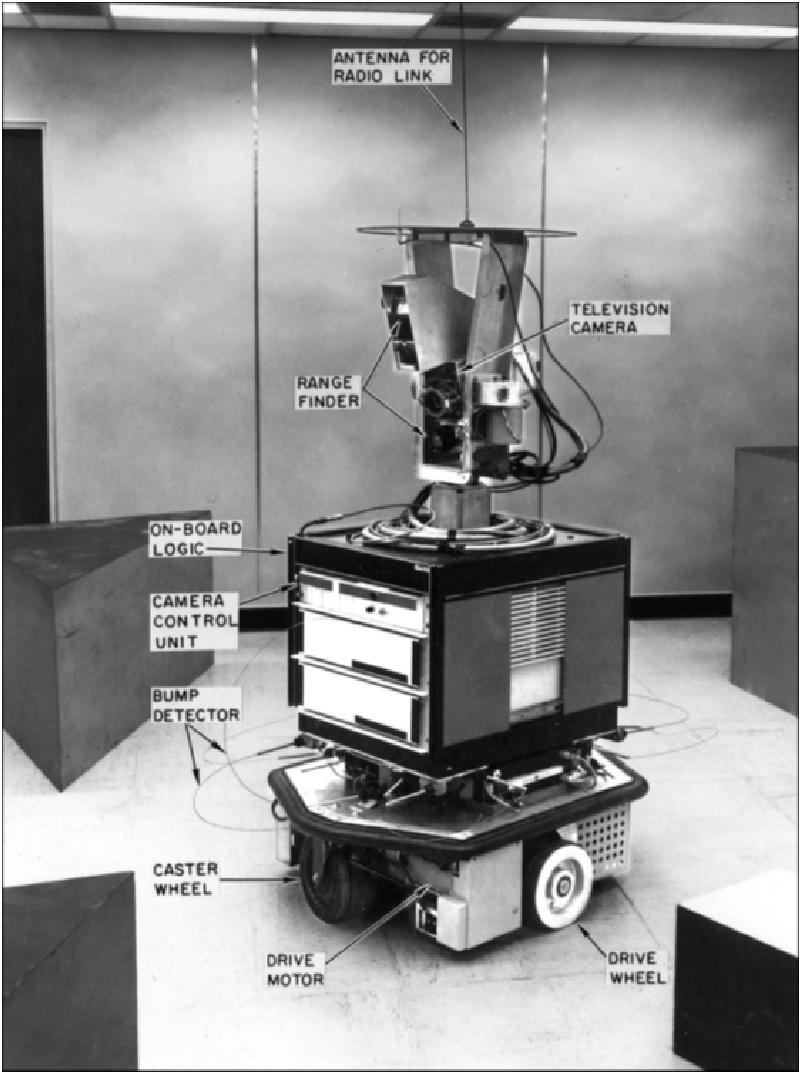
\includegraphics[width=\linewidth]{gaussian_map_5x5_sigma_1.5}
        \caption{$\sigma=1.5$}  
    \end{subfigure}
    % \hfill
    \begin{subfigure}[h]{0.115\textwidth}
        \centering
        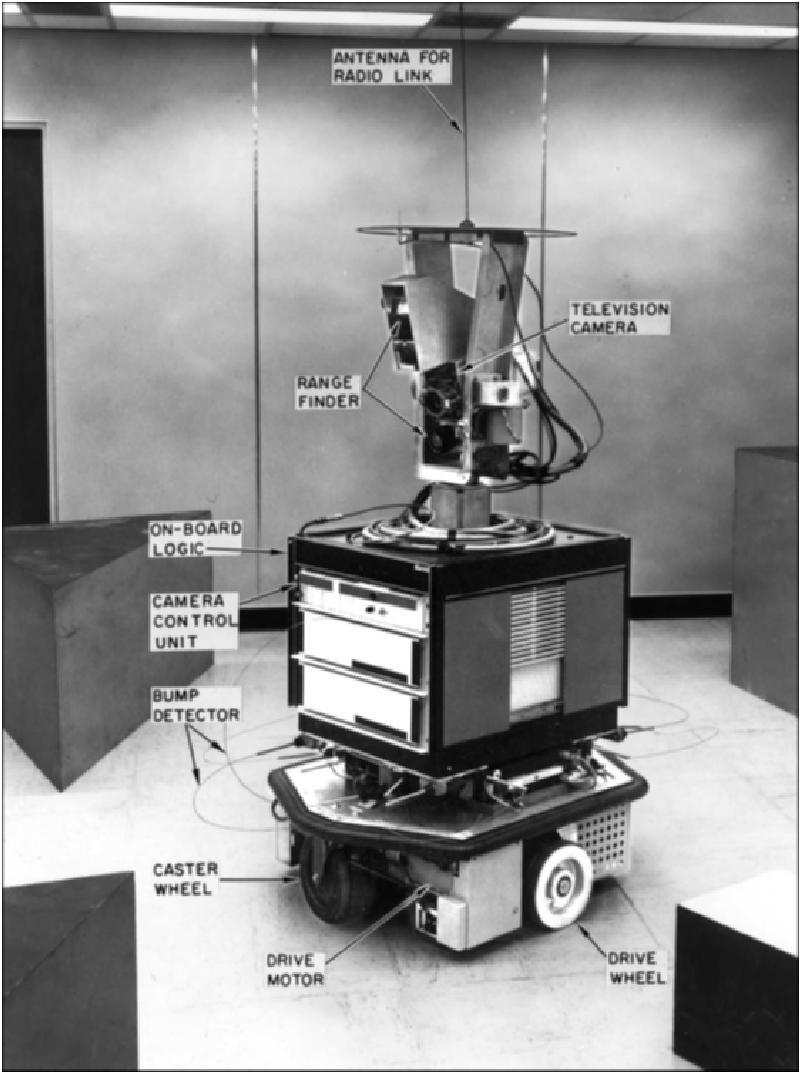
\includegraphics[width=\linewidth]{gaussian_map_5x5_sigma_3}
        \caption{$\sigma=3.0$}  
    \end{subfigure}
    \begin{subfigure}[h]{0.115\textwidth}
        \centering 
        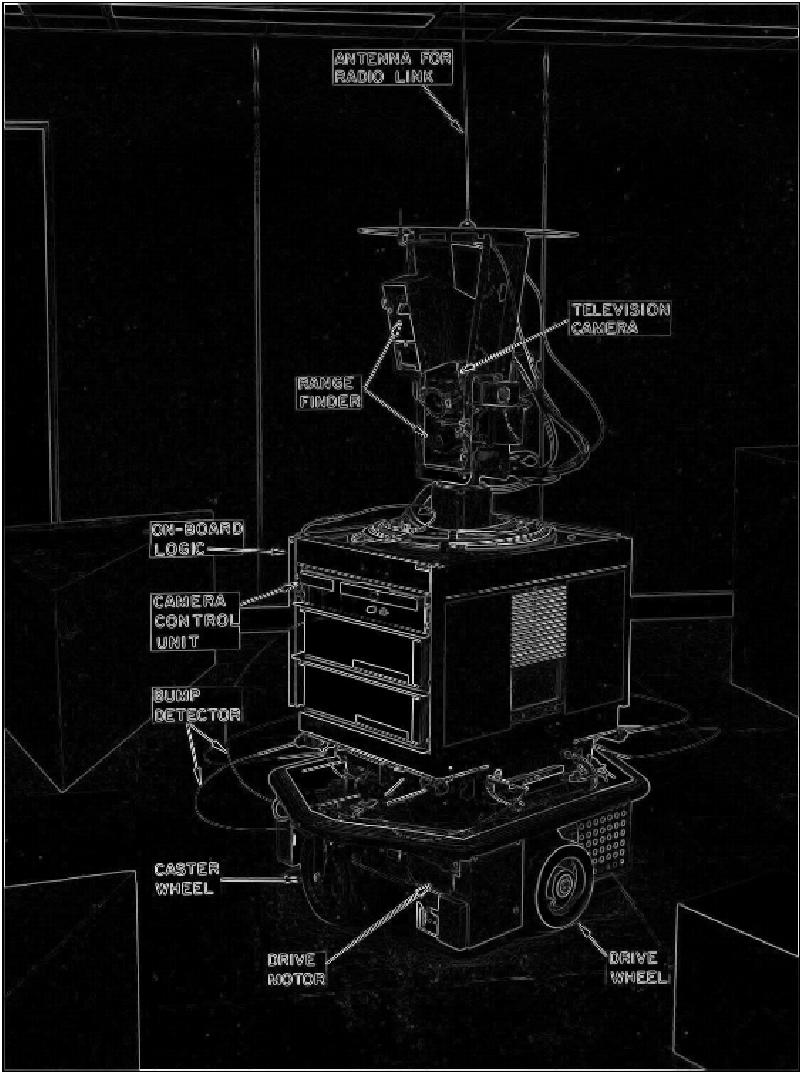
\includegraphics[width=\linewidth]{gaussian_edge_map_5x5_sigma_0.1}
        \caption{$\sigma=0.1$}  
    \end{subfigure}
    % \hfill
    \begin{subfigure}[h]{0.115\textwidth}
        \centering 
        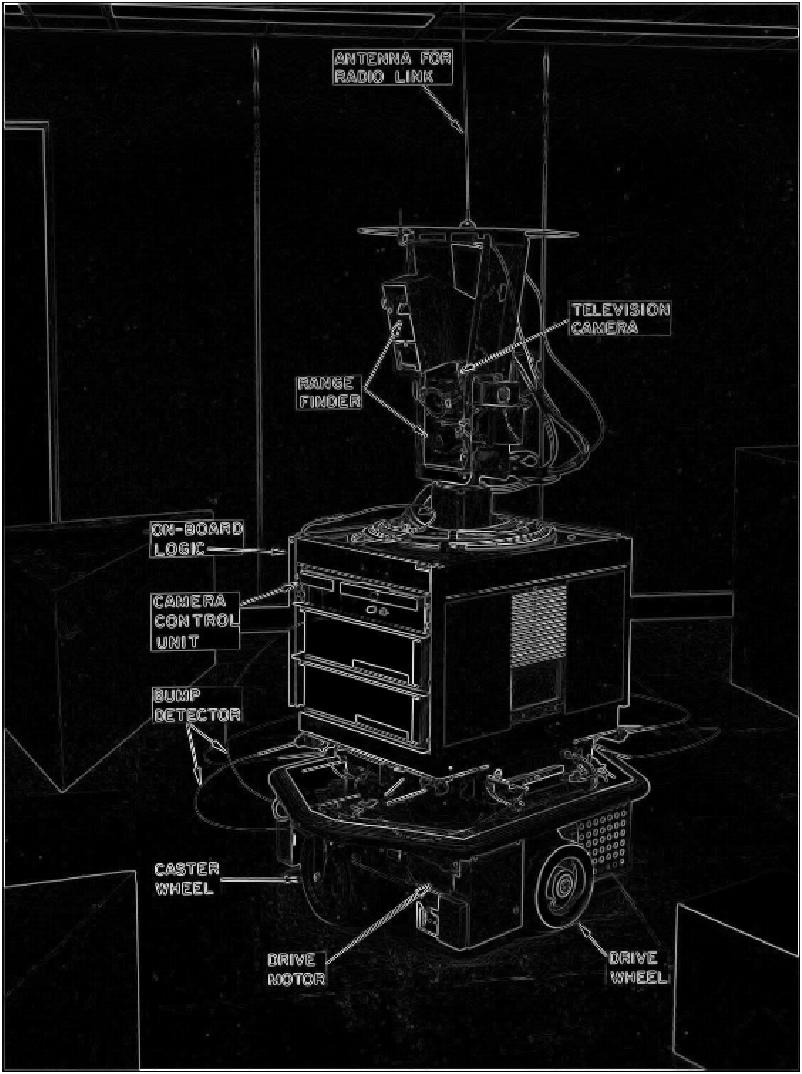
\includegraphics[width=\linewidth]{gaussian_edge_map_5x5_sigma_0.5}
        \caption{$\sigma=0.5$}  
    \end{subfigure}
    % \hfill
    \begin{subfigure}[h]{0.115\textwidth}
        \centering
        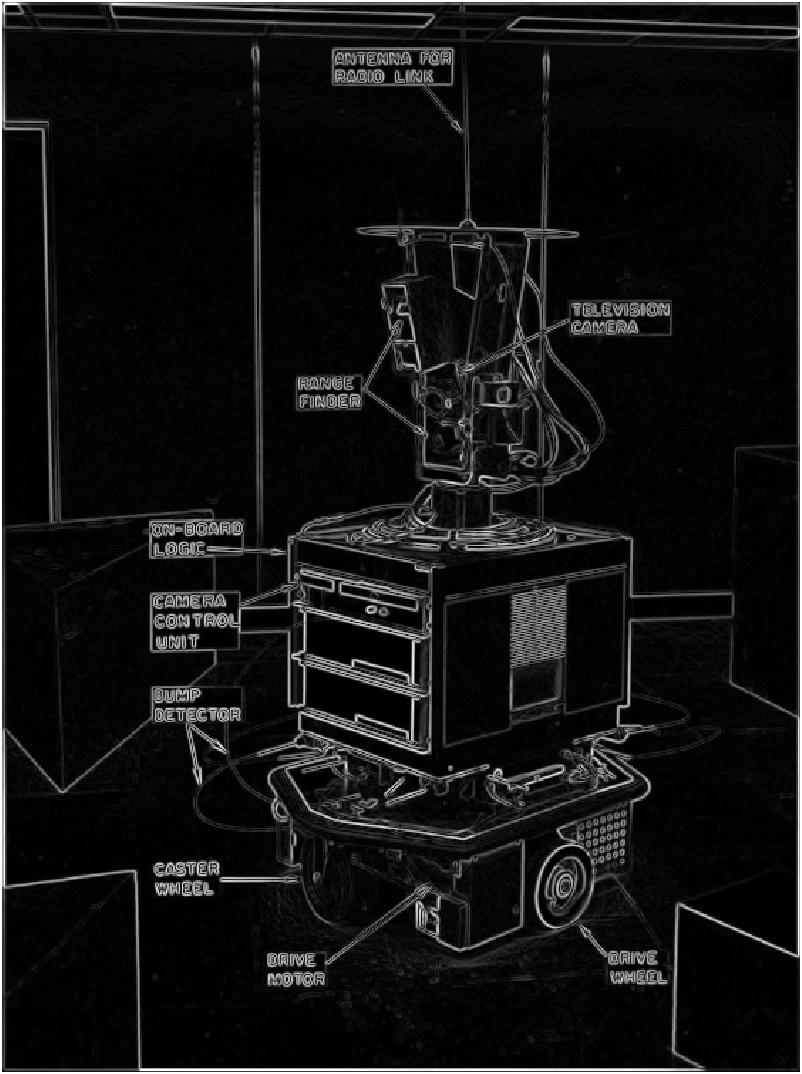
\includegraphics[width=\linewidth]{gaussian_edge_map_5x5_sigma_1.5}
        \caption{$\sigma=1.5$}  
    \end{subfigure}
    % \hfill
    \begin{subfigure}[h]{0.115\textwidth}
        \centering
        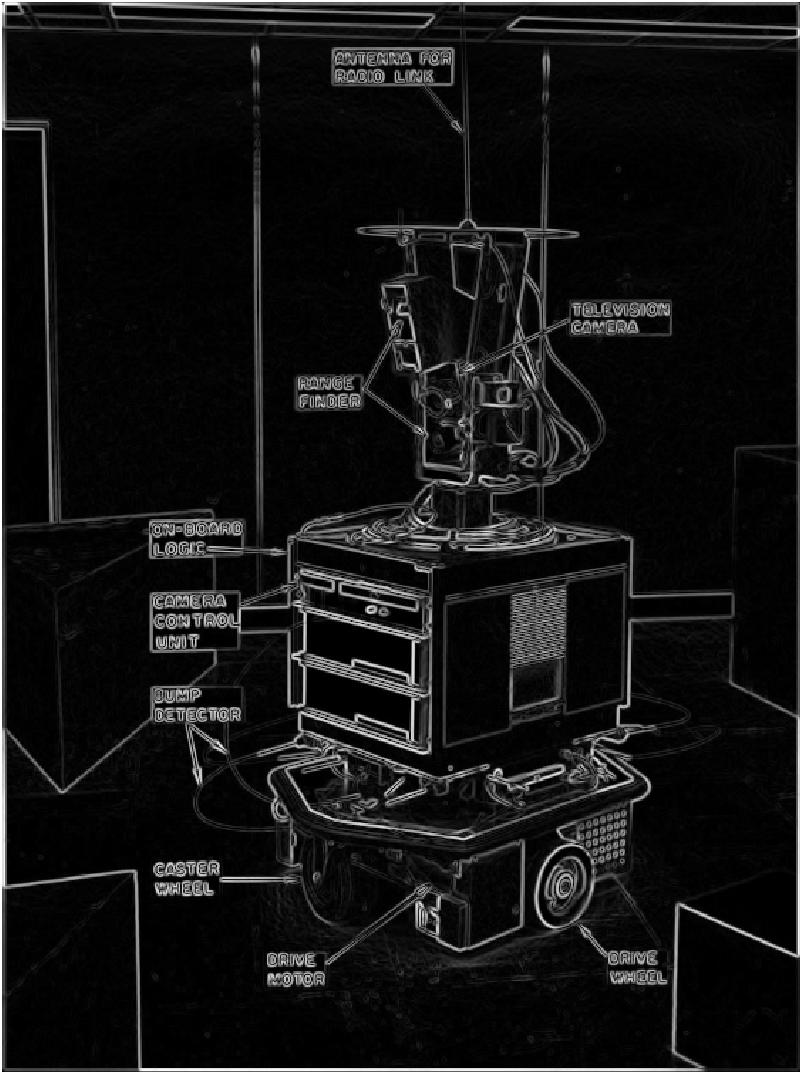
\includegraphics[width=\linewidth]{gaussian_edge_map_5x5_sigma_3}
        \caption{$\sigma=3.0$}  
    \end{subfigure}
    \caption{Experiments with different $\sigma$ values while keeping the filter size 5x5. The top row contains pure images on which the Gaussian filters were applied. The bottom row contains the top row images but on which the horizontal and vertical Sobel filters were applied and the magnitude was calculated}
    \label{fig:4}
\end{figure}

\noindent\textbf{Task}: now apply gradient operators such as the Sobel operators to the  blurred images.

\hfill

\noindent\textbf{Results}: the results can be seen in bottom rows of \autoref{fig:3} and \autoref{fig:4}. They compliment the explanation in \autoref{subsection:1:2} where a trade-off between edge details and noise was mentioned.

\hfill

\noindent\textbf{Question}: what happens to the edges in the heavily blurred case after applying gradient operators, such as Sobel operators?

\hfill

\noindent\textbf{Answer}: thicker edges stand out more and thinner edges almost disappear. This is because thin edges may sometime be confused with noise which gets averaged out after heavily blurying an image. Strong edges, on the other hand remain standing out therefore the gradient operator captures the changes and emphasizes them.

\begin{figure}[h]
    \centering 
    \begin{subfigure}[h]{0.155\textwidth}
        \centering 
        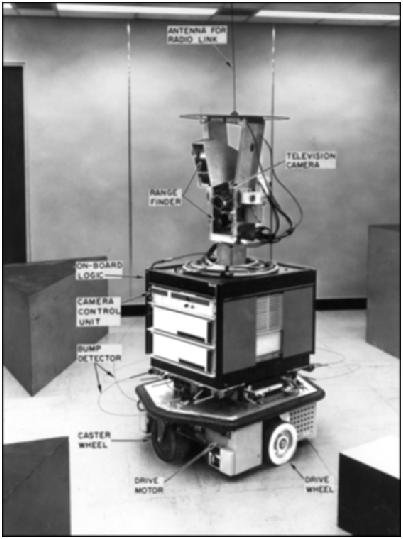
\includegraphics[width=\linewidth]{heavy_blur}
        \caption{Gaussian}  
    \end{subfigure}
    % \hfill
    \begin{subfigure}[h]{0.155\textwidth}
        \centering 
        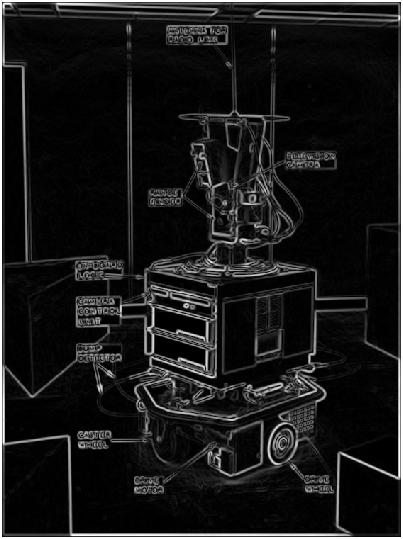
\includegraphics[width=\linewidth]{heavy_blur_9x9_sigma_3_magnitude}
        \caption{Sobel}  
    \end{subfigure}
    % \hfill
    \begin{subfigure}[h]{0.155\textwidth}
        \centering
        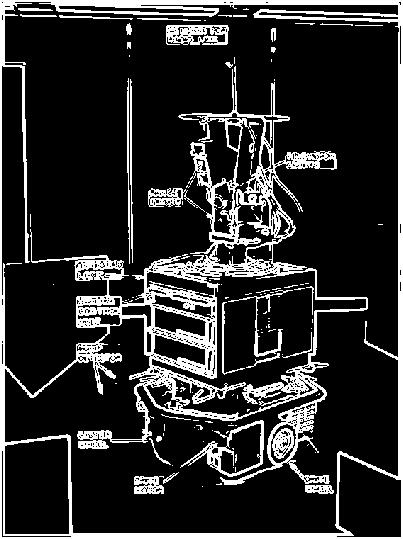
\includegraphics[width=\linewidth]{heavy_blur_9x9_sigma_3_edges}
        \caption{Threshold}  
    \end{subfigure}
    % \hfill 
    \caption{A heavily blurred image with a Gaussian filter of size 9x9 and $\sigma=3$. The magnitude of the Sobel operators was computed and the acquired map was thresholded at 40}
    \label{fig:5}
\end{figure}

\subsection{Task 2}
\noindent Task 2 just asks some reassurance questions to which the explanations could mainly be applied from the previous subsection.

\hfill

\noindent\textbf{Question}: what is the effect of increasing the size of the Gaussian Filter (3x3 versus 5x5 for example)?

\hfill

\noindent\textbf{Answer}: this was answered in \autoref{subsection:2:1}. In the particular case of 3x3 vs 5x5, 3x3 filter leaves more details (thus more noise) than 5x5. So the image with 3x3 filter is less blurry. It can also be seen that, after applying the threshold, there are more false positives in the background captured, but also more true positives within thin edges.

\hfill

\noindent\textbf{Question}: what is the effect of changing the standard deviation \textbf{s} ($\sigma$)? Why do you see what you see?

\hfill

\noindent\textbf{Answer}: this was answered above in \autoref{subsection:2:1}.

\section{Analysis Part 3}
\subsection{Step 3}

\noindent Step 3 asks to check how the performance differs between applying 2 1D \emph{Gaussian} filters (in sequence - first, a horizontal filter over every image row, then a vertical filter over every image column) and 1 2D \emph{Gaussian} filter.

\hfill

\noindent\textbf{Question}: can you detect differences in the CPU times as the mask sizes increase?

\hfill

\noindent\textbf{Answer}: for small matrix size (3, 5 and 7) 1 2D convolution performs faster than 2 1D convolutions. However for the kernel sizes of 9 and above, the time taken to perform the convolution for a 2D case dramatically increases compared to 1D case (e.g., twice the duration when filter size is 15).

\begin{figure}[h]
    \centering
    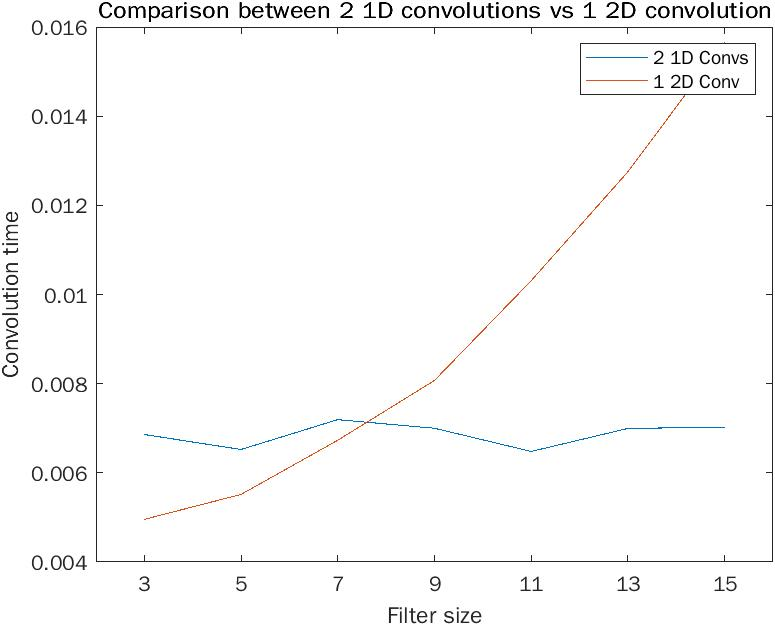
\includegraphics[width=\linewidth]{2d_vs_1d}
    \caption{A comparison of time taken to perform full convolution between applying 2 1D Gaussian filters and 1 2D Gaussian filter}
    \label{fig:6}
\end{figure}

\noindent\textbf{Question}: are there any effects due to small floating point errors?

\hfill

\noindent\textbf{Answer}: there are very small relative errors, i.e., the range is from $10^{-16}$ to $10^{-18}$. This means the convolution result is almost the same.

\subsection{Step 4}\label{subsection:3:2}

\noindent Step 4 asks to produce an edge map after applying a \emph{Laplacian} filter where edges are determined by \emph{zerocrossing}.

\begin{figure}[h]
    \centering 
     
    \begin{subfigure}[h]{0.23\textwidth}
        \centering 
        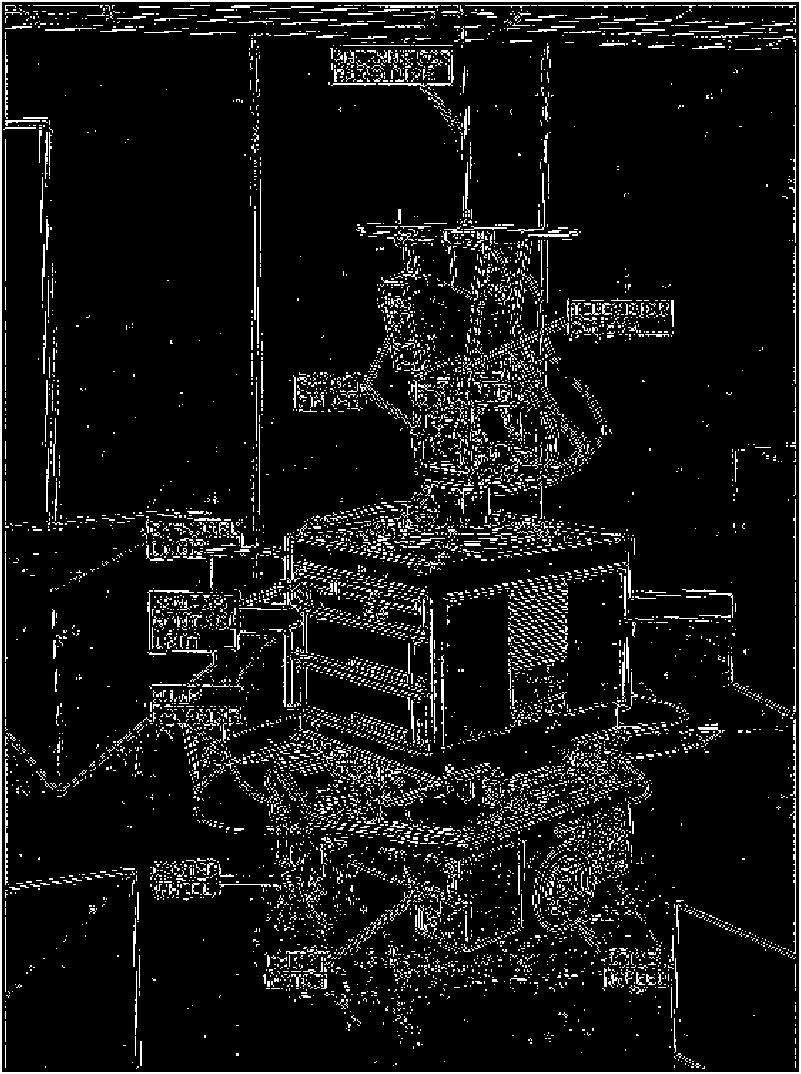
\includegraphics[width=\linewidth]{laplacian_zerocross}
        \caption{Laplacian + zerocross}  
    \end{subfigure}
    % \hfill
    \begin{subfigure}[h]{0.23\textwidth}
        \centering
        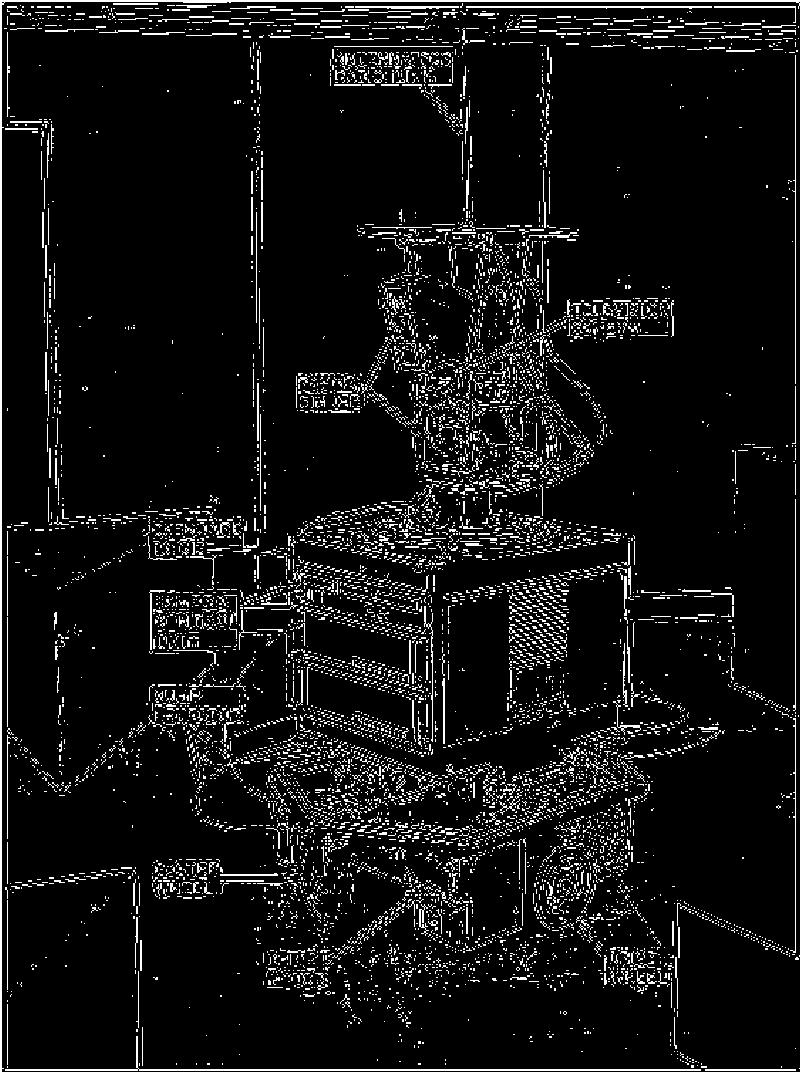
\includegraphics[width=\linewidth]{log_zerocross}
        \caption{LoG + zerocross}  
    \end{subfigure}
    % \hfill 
    \caption{Second order gradient inspection method to determine the edges: Laplacian is applied to the first image and Laplacian of Gaussian (Laplacian convolved over 5x5 Gaussian filter) to the second one. Edges are determined by zerocrossing}
    \label{fig:7}
\end{figure}

\noindent\textbf{Question}: why does it produce a poor result compared to the other operators?

\hfill

\noindent\textbf{Answer}: the poor result is due to finite difference approximation. In other words, it is not always clear where exactly the edge is, it could be one pixel further or closer. It is because zero crossing determines a thin line between pixels with values with opposing signs and the values themselves could be close to 0 meaning higher uncertainty.

\subsection{Task 3}

\noindent Task 3 asks to produce a \textbf{Laplacian of Gaussian} operator and see how it affect the image.

\hfill

\noindent\textbf{Question}: How could you combine the idea of the \emph{Laplacian} operator with the idea of \emph{Gaussian} smoothing?

\hfill

\noindent\textbf{Answer}: first we find the gradient of the \emph{Gaussian} kernel (via convolution with \emph{Laplacian} filter). Then we take the \textbf{LoG} filter, apply it to the image and then apply the \emph{zerocrossing} to determine the edges. It still doesn't produce great results due to the reason in \autoref{subsection:3:2}. The result and comparison with a pure \emph{Laplacian} can be seen in \autoref{fig:7}.


\begin{thebibliography}{1}
\bibliographystyle{IEEEtran}

\bibitem{ref1}
Canny, J., {\it{A Computational Approach To Edge Detection}}, IEEE Transactions on Pattern Analysis and Machine Intelligence, 8(6):679–698, 1986.

\bibitem{ref2}
Leventhal, Daniel (Autumn 2011). "Image processing". University of Washington. Retrieved 2019-12-01.

\end{thebibliography}

\end{document}